\section{ FaceLift  Specifics}
We now delve deeper into the specific implementation of the pipeline described before for the use case of FaceLift, which is a beautification framework for urban images. This section will walk through the data that we use for this implementation and the evaluation of the proposed pipeline in the context of urban image beautification.

%Looking at diminished classifier performance for city only images augmented using translation and rotation, the question arises, which images are worth augmenting, and which images, when augmented, add more noise to the system than information. 
%On these lines, we look at a sample set of images, which are augmented at varying distances of 0, 20, 40 and 60 meters. A simple similarity metric of cosine angle between Fc7 features of images (Placesnet) is used to computationally validate similarity. 
%Figure \ref{fig:normedCosine} suggests that on an average across the sample set, the similarity tends to go down (Angle tends to increase) as you go farther from the original image. But all is not lost as the standard deviation suggests that even at 60 meters, you may find images which are similar at par to the one taken at 0 meters translations.

\subsection{Data }
\label{sec:label}
%For FaceLift, we build on the data annotated as a part of a study about 
Our seed dataset comes from StreetScore, a research work on urban affects scores \cite{naik2014streetscore}. The dataset in total contains 11183 images across the world from Google StreetView. The images are compared in a pairwise manner for qualities such as beauty, depression, richness , safety etc. For the purpose of our paper, we use the annotations for beauty. To train our classifier $C$ to detect beauty in terms of categories $Y$, we need to transform pairwise votes into absolute scores, then discretize absolute scores into a finite set of categories $y_i$. We transform the pairwise votes %from the dataset are then transformed 
into ordinal scores using the TrueSkill \cite{herbrich2007trueskill} algorithm. %This allows us to subsequently separate annotated images into classes of high confidence based on the number of votes the image has got.  
To ensure reliability of absolute judgements, we filter out images with less than 3 votes.
To discretize the resulting scores, we heuristically partition the data into two classes with maximum separation. Figure \ref{fig:Trueskill} shows the distribution of Trueskill score estimates with the threshold scores at which we decide beauty or ugly class boundary. 
%\textbf{[CHANGE IMAGE TO SHOW WHERE THE THRESHOLDS ARE]}
 
\begin{figure}[ht]
	\centering
	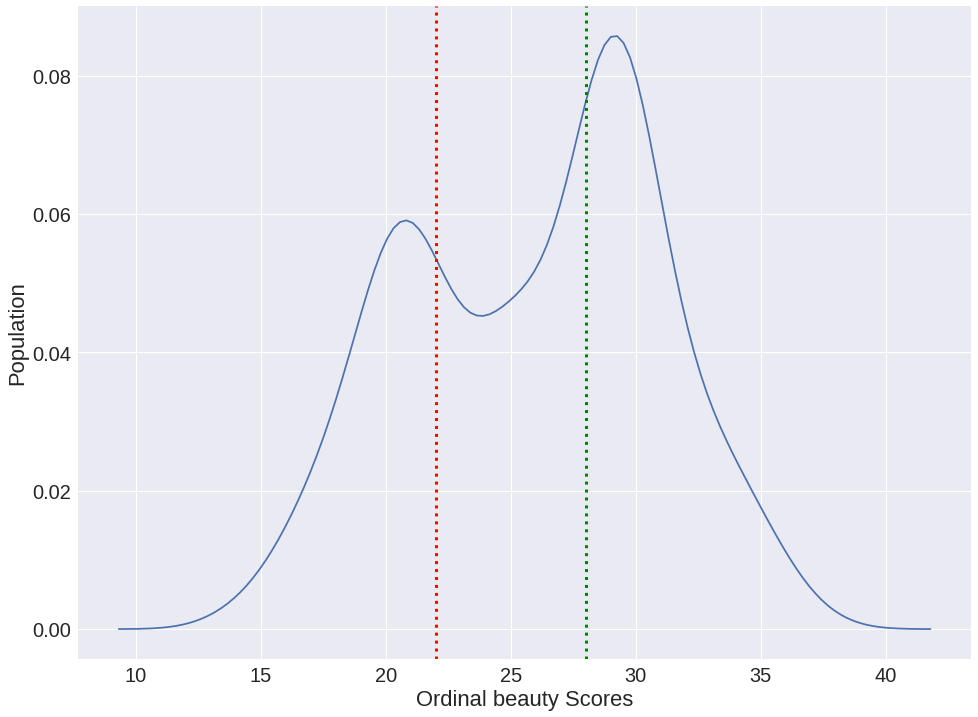
\includegraphics[width=0.8\columnwidth]{Plot/Trueskill.png}
	\caption{Distribution of ordinal scores for images with at-least 4 votes. The red and green line represent the threshold below and above which images are tagged Ugly or beautiful. Images in between are dropped for separability }
	\label{fig:Trueskill}
\end{figure}


%\textbf{[Where is the Clustering part??]}

\subsection{Classifying Beauty}
%As mentioned before, the quantity of annotated data for such a use case is extremely sparse. 
\subsubsection{Augmentation similarity bound}
\label{sec:bound}
Despite over a hundred thousand images in the original data, after filtering we are left with 20,000 images only.
This is non-ideal to train classifiers with substantial number of parameters such as convolutional neural networks.
Hence we choose to augment the dataset by exploiting the geo-located nature of the image dataset. 
With an assumption that "\textbf{[A1]}\textit{rotation of camera, keeping the location constant, does not change the composition of the image considerably}" we now have two sets of images. 
First set  is $R(i) \forall i \in I$ , which consists of images acquired by just rotating the pitch for a given annotated image. We rotate the camera across different values $\theta \in {-30^{\circ}, -15^{\circ} , 15^{\circ} , 30^{\circ} }$. For these images, the beauty score can be safely transferred from $i$. 
Next we  acquire set of Images $T(i) \forall i \in I$, from a near geographic vicinity of a StreetView image $i$ in the StreetScore datase, by translating the streetview  camera at distances of 10, 20 40 and 60 meters. 
%We also acquire images at variable angle of rotation $\theta \in {-30^{\circ}, -15^{\circ} , 15^{\circ} , 30^{\circ} }$, keeping the yaw axis of the camera constant.%, %as well as 
%of the annotated image.
%To evaluate this bound, we test a smart augmentation protocol. We augment each image in our seed dataset, %we collect additional images for each image in the base dataset of 20k 
%by translating the street-view camera from the original image location. The images are collected at various distance but with same pitch and rotation of camera, as the original image. We select 10, 20, 40 and 60 meters as candidates for translation of camera. 
We then represent each image from both sets, using features from the last but one layer of PlacesNet \cite{zhou2014learning}. We then calculate a set of cosine similarities $ S_t = \{s(i,T(i)) \forall i \in I \}$
between each original image $i$ and all images in the augmented set $T(i)$. 
We also calculate another set of cosine similaritie  $ S_r = \{s(i,R(i)) \forall i \in I \}$
Now with assumption \textbf{[A1]} , we only select translational images in the augmentation set where $s(i,T(i)) < median(S_r)$. This implies that the translational images  $T(i) $ are just as similar to the original annotated image, as images acquired by rotation of camera. 
Hence we arrive at a similarity bound
\begin{equation}
	\rho = median(S_r) \text{ where }{S_r} = \{s(i,R(i)) \forall i \in I \}
	\label{eq:bound}
\end{equation}

%Similarly, we collect a set $R(I)$ containing pictures taken at the I location but with \textbf{[SAY ANGLES]} rotation, and compute $s(I,R(I))$ as the similarity values between I and images in R. %$ of the augmented images. 
%\textbf{[ASSUMPTION SAy why R(I) is augmentable]}
% We then create 2 image sets:
 
 %separate the set of orginal and Augmented images into two sets as follows: 
 
\subsubsection{Semantics of Augmentable images}
Given that we now had a similarity bound to decide whether to augment or not a particular image, we wondered whether certain types of scenes are more prone to augmentation compared to others.  So we partitioned our data in two sets
\begin{itemize}
	\item $set A$: contains images where the median similarity  between translated images and the original image ${s(i,T(i))} < \rho$ .
	
	\item $set B$:  Images whose similarity with their translated set is farther apart i.e. ${s(i,T(i))} > \rho$ .
\end{itemize}

%\textbf{[Conclusion on why A is augmentable and B is not]} 

We describe each image in both sets according to the scene depicted, by collecting the PlacesNet \cite{zhou2014learning} labels with the top5 confidence scores. We then aggregate such labels at a set level by computing a TF-IDF metric. The resulting set of \{label,Count\} pairs are essentially how common or uncommon is a particular scene label in $setA$ compared to $setB$ 


% for each image for both sets, and find the prevalence of labels in both the sets after balancing them. This is done simply by subtracting $\{L_i   \forall i \in A\}$ where $L_i$ is the label. The resulting set of \{label,Count\} pairs are essentially how common or uncommon is a particular scene label in $setA$ compared to $setB$
%To analyse types of scenes that fall in each set, we first get the top 5 PlacesNet \cite{zhou2014learning} labels for each image for both sets, and find the prevalence of labels in both the sets after balancing them. This is done simply by subtracting $\{L_i   \forall i \in A\}$ where $L_i$ is the label. The resulting set of \{label,Count\} pairs are essentially how common or uncommon is a particular scene label in $setA$ compared to $setB$
%\begin{figure}[ht]
%	\centering
%	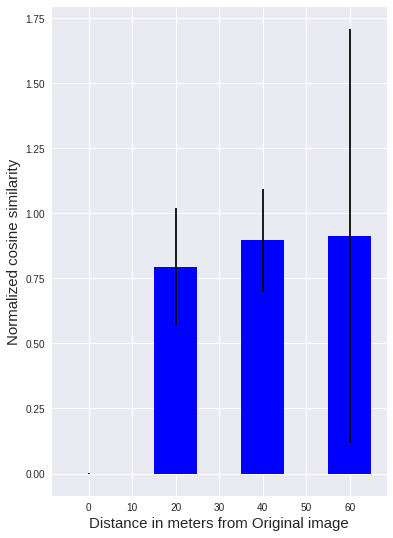
\includegraphics[width=0.5\columnwidth]{Plot/Normed_cosineSim_Aug_5000.png}
%	\caption{Variation of similarity angle (radians) with deviations}
%	\label{fig:normedCosine}
%\end{figure}

\begin{figure}[ht]
	\centering
	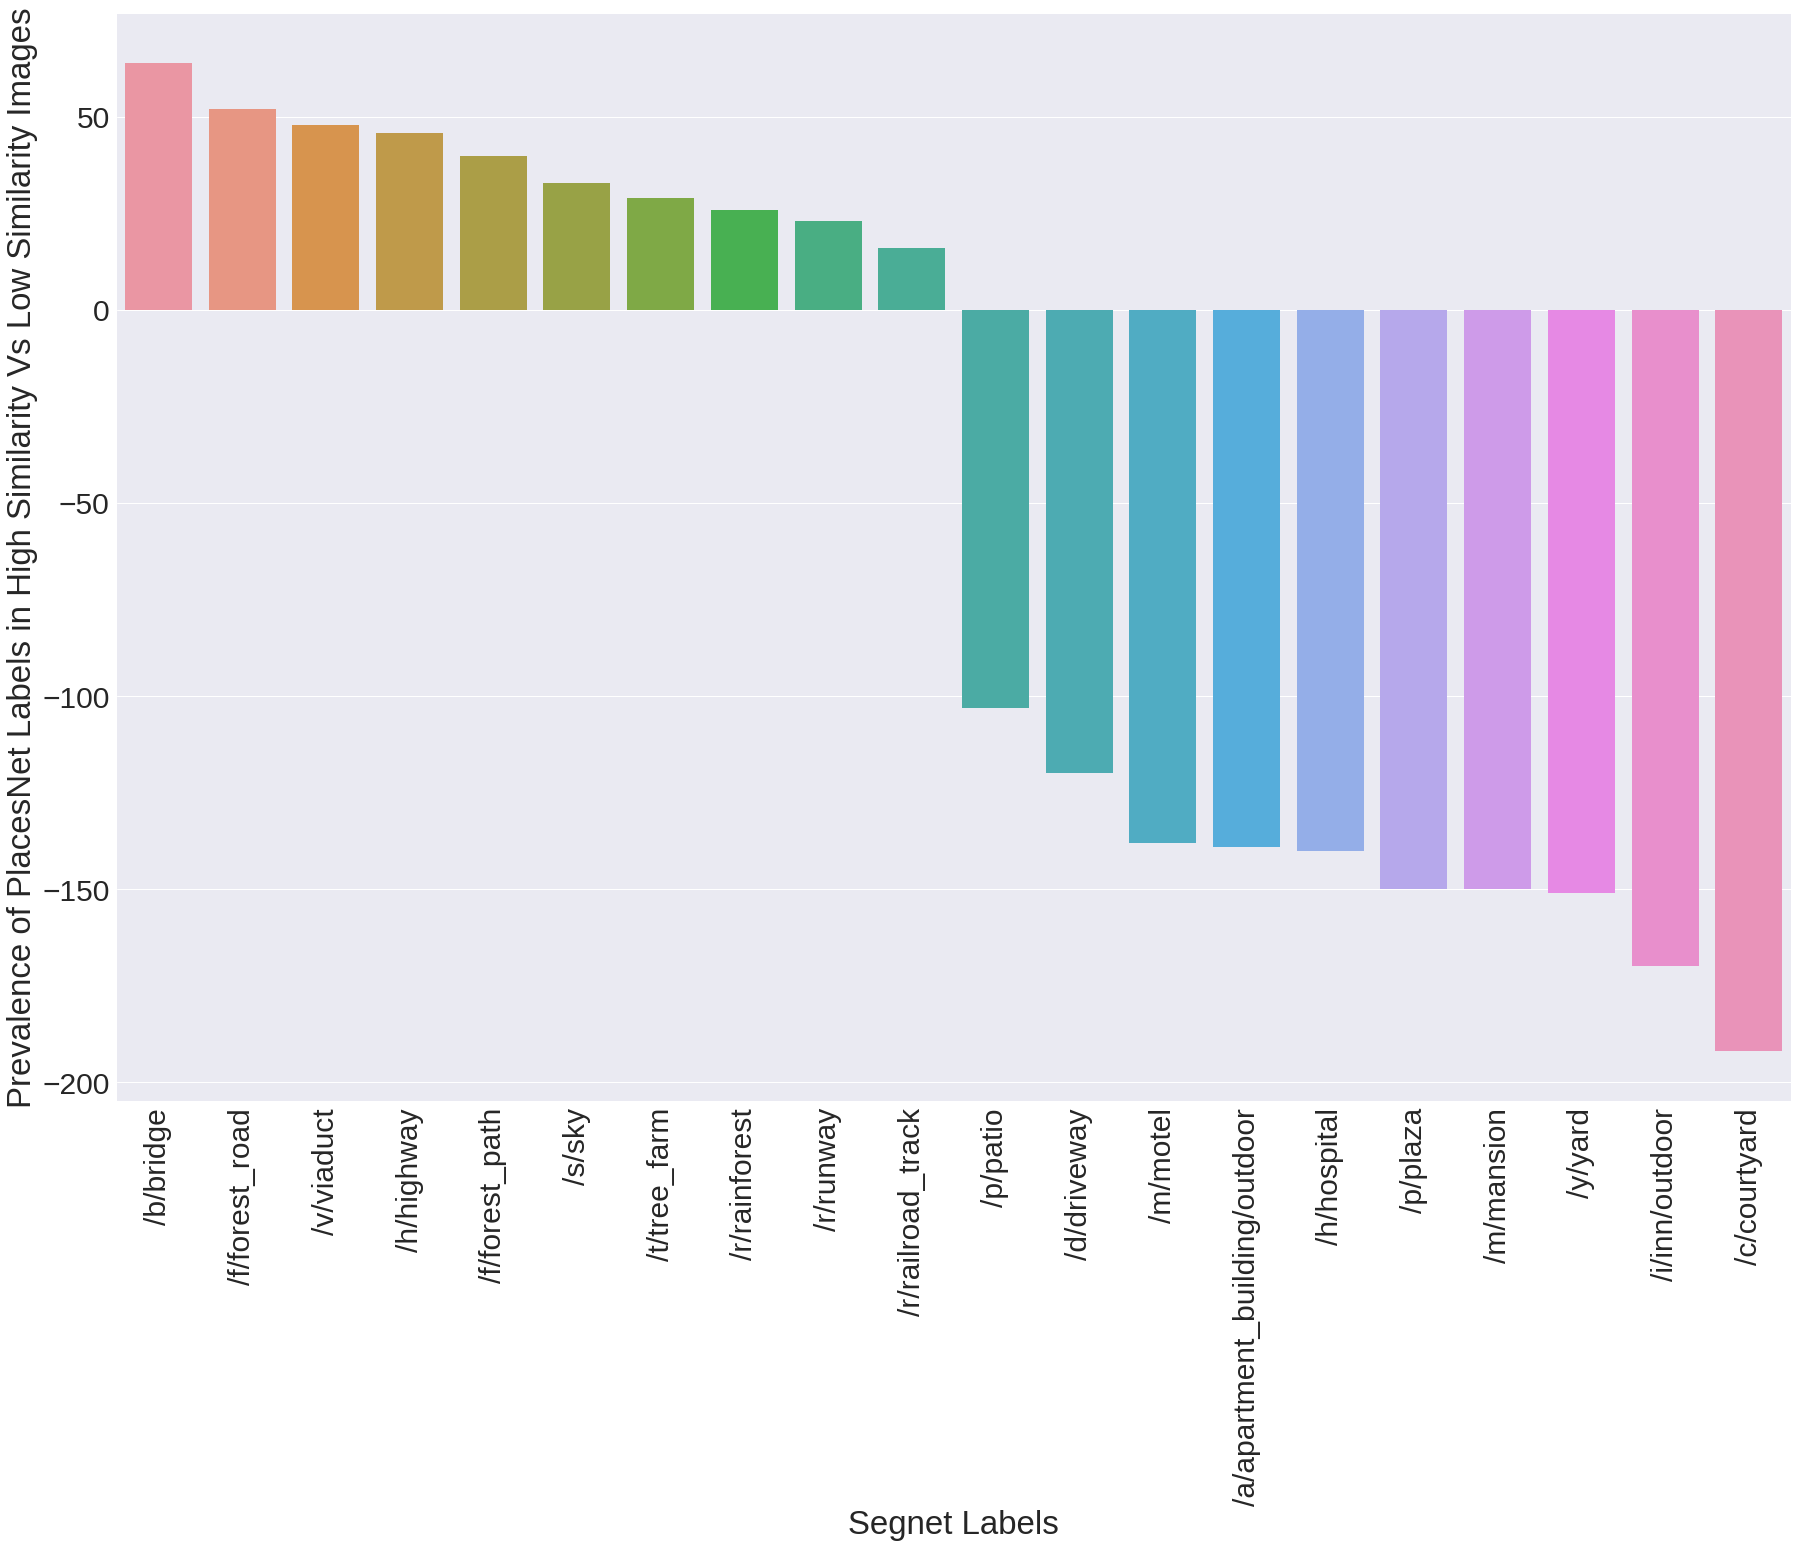
\includegraphics[width=\columnwidth]{Plot/SimilarityPlacesPrevalence.png}
	\caption{Prevalence plot of types of scenes prevalent in Similar images compared to dissimilar ones.}
	\label{fig:augmentationSimilarity}
\end{figure}

The resulting prevalences of scene types can be seen in Fig \ref{fig:augmentationSimilarity}. The plot shows that scenes like highways, fields and bridges, typically more uniform and open, 
don't change despite translation. On the other hand, there are more urban scenes like gardens, residential neighbourhoods , plazas and skyscrapers which are intuitively more sensitive to change in perspective by translation. 

\subsubsection{Beauty Classifier with Smart Augmentation}
We employ the above observations to train the beauty classifier model. We start with  the base dataset of 20k images, as described in Section \ref{sec:label}. We then progressively augment the data: first with rotation across 5 angles, then rotation with uniform translation for all images, and then rotation and translation for only images which satisfy similarity bound as evaluated as shown in Equation \ref{eq:bound}. 
We then train a Convolutional neural net model based on AlexNet architecture \cite{szegedy2015going} on each of these augmentated datasets. The training is done on 70\% split of the data and tested on the 30\%. 

We see considerable improvement in classifier accuracy \ref{tab:classifier}, with the best model performing at 73\% accuracy for classifying images in two classes of Beauty and Ugly. 
This model represents the knowledge of the affective concept of beauty, learned from annotated and augmented streetview images. 


\begin{table}[h]
	\centering
	\begin{tabular}{|c|c|}
		\hline
		\textbf{Policy} & \textbf{Accuracy (Percentage)}\\
		\hline
		No augmentation & 63 \\
		\hline
		Rotation only & 68 \\
		\hline
		Rotation + translation  & 64 \\
		\hline
		Rotation + Smart Translation & 73.5 \\
		\hline
		
		\hline
	\end{tabular}
	\caption{Performance differences based on different augmentation policies, for the 3 Cities data}
	\label{tab:classifier}
	%        \vspace{-5mm}
\end{table}


\subsection{Generating Beauty}
% \textbf{[Add GAN retraining process + crappy image comparison, possibly split into Generating and Retreving dedicated subsections.]} 
Once we learn a reliable model for beauty from the data, we need to employ generative models along with a way to change input codes to the GAN, so as to maximize beauty content in an a-priori (ugly) image. This is done in two steps. 

\subsubsection{Generator}
Generative Adverserial networks are an extremly useful tool when it comes to generating samples from a learned distribution\cite{radford2015unsupervised}. GANs work by learning a pair of networks where one learns the distribution of sample space and generates samples using de-convolutional layers and another learns to discriminate between natural images from the training set and synthetic images generated by the generators. The problem is a min-max arrangement where we want to maximize error in discriminator by minimizing error between generated and natural images, there by generating samples that confuse the discriminator. But GANs are known to be very tricky to train \cite{gulrajani2017improved} and hence to our end, we first try to use a pre-trained GANs on Imagenet images from \cite{nguyen2016synthesizing}. We use this GAN to generate images for maximizing beauty, but because of the vast difference in the ImageNet image distributions for the 1000 classes, and the streetview images, the results were not very optimal. This provoked us to retrain the generator on the training dataset we used for Classification model. This improved the GAN performance considerably and it started generating images which do not entirely resemble natural streetview images, but look like paintings of these scenes. 

\subsubsection{Activation Maximization}
We build on top of the activation maximization technique elaborated by Nguyen et. al \cite{nguyen2016synthesizing} which utilizes the property of locality of codes with respected to generated images in Generator networks. Which means Generator codes which are close to each other would create similar looking images.This approach was initially aimed at visualizing the learnt knowledge of a convolutional neural network classifier. This is done by maximizing the activation of a particular output class probability neuron in a trained Classifier network, by feeding it images generated by a generator network. The maximization is achieved by doing gradient descent on the input generator codes with respect to the classifier neuron activation, keeping everything else locked. The result is a synthetic image that has a high activation for a pre-determined output neuron.
To our end, we modify this method by starting the maximization method from a code which is closest to the a-priori input image, which is the ugly urban image. This initializes the generator to a point from which the modified image should be ideally closest in terms of composition to the a-priori image. We then maximize the Beauty neuron of our trained classifier by doing the activation maximization process on the initialized generator, and stop as soon as the generated image pixels start getting saturated. The resulting output image is a natural-like image, which maximizes the beauty neuron for our classifier. We hypothesize that because the process begins from an a-priori image, the resulting image is closest possible template to the ugly input image, but with the beauty affect maximized. 
%We generate template images for randomly chosen 500 most ugly and 500 most beautiful images from the dataset. We then transform them using the Activation maximization and retrieval. The details of retrieval function are elaborated in the next subsection.


%modify the Activation maximization algorithm from \cite{nguyen2016synthesizing}. As described in Section \ref{sec:Pipeline}, we generate the template images for randomly chosen 500 most ugly and 500 most beautiful images from the dataset. We then transform them using the Activation maximization and retrieval. Figure \ref{fig:BeautyExample} shows one such beautification example with the synthetically created Template.

\begin{figure*}[h]
	\centering
	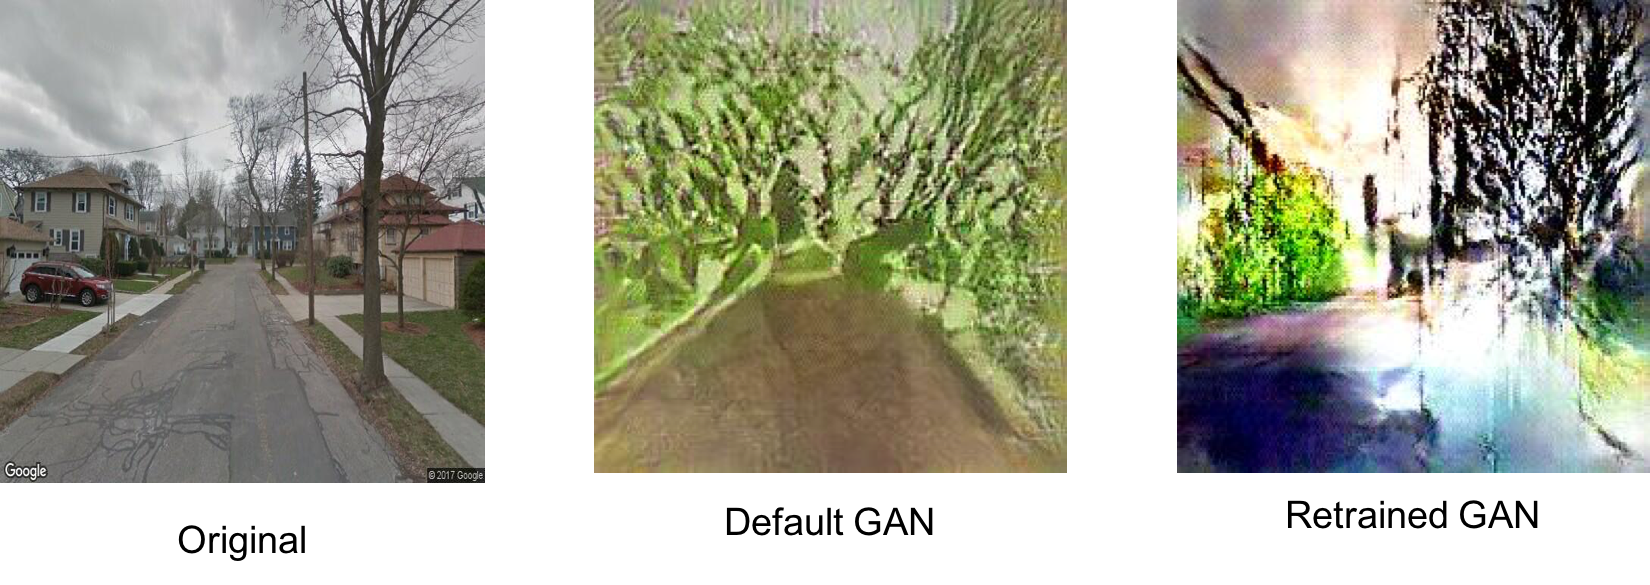
\includegraphics[width=0.7\linewidth]{Plot/GanCompare.png}
	\caption{Comparison of using the Default ImageNet GAN against Custom trained GAN for Activation maximization. By re-training the GAN on the test dataset, we can see improvement in terms of structure and colours in the generated images}
	\label{fig:BeautyExample}
\end{figure*}


\subsection{Retrieval of beauty}
Once we have a template from the Activation maximization, we need a way to translate the template into an image that looks very natural. We decided to go the Retrieval route. This formulates the problem as retrieving an image from a hash of the information. In our case the hash is the template that is generated by the generator so as to maximize beauty in the a-priori image. We use a pre-trained deep  network, which is trained to classify Scene types to a very high accuracy \cite{zhou2014learning}. We use the last but one fully connected layer of this network to extract a 4096 dimensional feature vector from the template image. We then extract similar feature vectors from the complete test dataset. We can now use the $L_2$ Norm to find pairwise distances in the $R^{4096}$. Formally with $N$ test natural images and a template image $\hat{i}$ we extract $v_{\hat{i}} \in R^{4096}$ and and find pairwise distances  $\{d_j \text{  }\forall j \in N\} \text{ where } d_j = L_2(v_j , v_{\hat{i}})$ 
We then find the target image by finding the $min(\{d_j\})$. For the sake of redundancy, we find the top 5 such matches for every template $\hat{i}$ generated from every ugly image $i$. These target images are what we call the transformed images for maximizing beauty

\begin{figure*}[h]
	\centering
	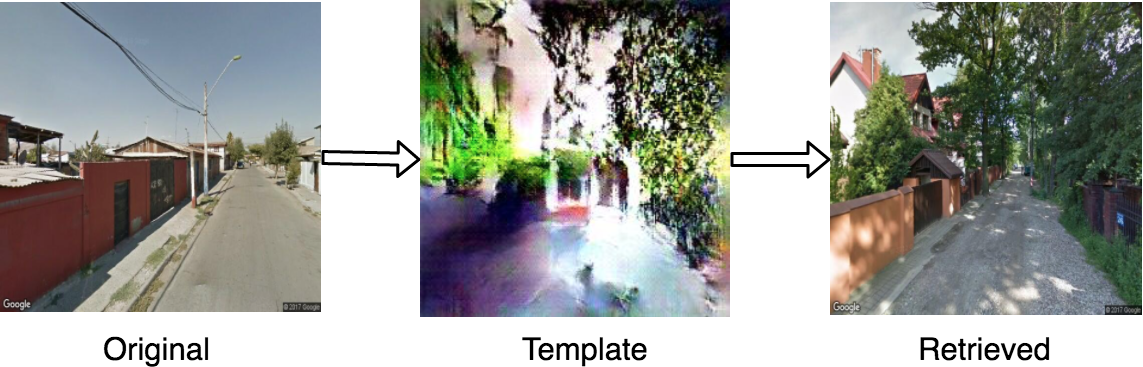
\includegraphics[width=0.7\linewidth]{Plot/Example.png}
	\caption{Example of Beautification Process}
	\label{fig:BeautyExample}
\end{figure*}

\subsection{Pipeline Validation}
\textbf{[add EXP details! number of participants, agreement, pay, and ground truth construction ...]}

Because beauty is a subjective opinion, we need to understand if our pipeline is able to actually learn and generate the intangible qualities of beauty. For this, we run a user study to check how often humans agree with the machine's inference. For this reason, we take help of crowd-sourcing to understand how much do real humans agree with the pipeline's transformations.
We randomly select 200 images, 100 beautiful  and 100 ugly as per their TrueSkill scores. These images are then transformed into the opposite side of the spectrum of beauty using FaceLift. As a result, a beautiful image would be transformed into an ugly image and vice versa. Then we design an Amazon Mechanical Turk experiment, where we ask the turkers to choose the beautiful image between the original and the transformed images, without giving any hints of the transformation. We make sure that we have at least 3 votes on each image comparison, there by allowing us to choose majority voting. The results show that over all , the Turkers agree with the model \textbf{76.5\%} of the time. Besides the over all agreement, the turkers agree \textbf{70\%} of the time with the process of beautification and \textbf{86\%} of the time with uglyfication. These results were a testament to the fact that our pipeline is learning the concept of beauty and then doing agreeable transformations on images.  